\section{Gaussian process surrogate}

The most popular surrogate model is the Gaussian process, we will now understand model
in more detail. Typically, a probabilistic regression model is on the from 
$$y = f_w(x) + \epsilon$$
where weights are trained. $f$ could describe a linear model, $f(x) = w^Tx$ or a polynomial
$f(x) = w\cdot x^2$ etc. the performance of the regression model is very dependend on the 
regression model. The Gaussian process takes a completely different approach, its model $f$ does not
include any parameters. If we collect the data in a vector $\textbf{f} := [f(x_1),\dots,f(x_n)]$
then the GP assign it a multivariate normal distribution, 
$$\textbf{f} \sim \mathcal{N}(\bm{\mu}, \bm{\Sigma})$$

where $\bm{\mu}$ typically is $0$ and the covariance matrix, is depeneded on the input, $x_1, \dots, x_n$, 
 $$\bm{\Sigma} = c(\textbf{x}, \textbf{x}) = \begin{bmatrix}
    c(x_1,x_1) & \dots & c(x_1,x_n)\\
    \vdots& \ddots\\
    c(x_n,x_1) & \dots & c(x_n,x_n) \end{bmatrix}\hspace{1cm} c(x, y) := Matern(x,y)...$$ this means
that a realization of the vector $\textbf{f}$ is often close to 0 with a variance of the diagonal
$\bm{\Sigma}$, \todo{NO!! Change}but also with a correlation between the elements in $\textbf{f}$
given by the off-diagonals in $\bm{\Sigma}$. This is a very important ingredience of a GP, if
$c(x_1,x_2) \approx 1$ (assuming that the variances of $\textbf{f}$ is 1, then $\bm{\Sigma}$ is a
correlation error) then realizations of $\textbf{f}$ always lead to similar values of $f(x_1)$ and
$f(x_2)$ (this can be seen in Figure \ref{GP_illustration}). This encapsulates the idea of a GP: similarities
(could be distance or other measures) in $x$ should lead to similarities in $f(x)$. Now, in the case
of extending it to a regression model, we need to bring a unobserved $y_*$ for a arbitrary location
$x_*$ into the game. Prior to observing any data, we assume that the corresponding $f_*$ is
just a new element in the multivariate normal distribution, 
\begin{align}
    p(f_*,\textbf{f}|\textbf{x}) = \mathcal{N}\left(\begin{bmatrix}
        f_*\\ \textbf{f}
    \end{bmatrix} \middle| \begin{bmatrix}
        0\\ \textbf{0}
    \end{bmatrix}, \begin{bmatrix}
        c(x_*, x_*) & c(x_*,\textbf{x})\\
        c(\textbf{x}, x_*) & c(\textbf{x}, \textbf{x})
    \end{bmatrix} \right)
\end{align}
yielding many possible outcomes for $f_*$, but with an average $E[f_*] = 0$ and variance of $V[f_*]
= 1$. Note given a realization of $\textbf{f}$, then the distribution of $f_*$ is changed.
Fortunately, a multivariate normal distribution is easy to deal with: The conditional
distribution of $f_*$ given $\textbf{f}$ is, 
$$p(f_*|\textbf{x}, \textbf{f}) = \mathcal{N}(f_*|c(x_*, x_*)^{-1}c(x_*, \textbf{x})\textbf{f}, c(x_*, x_*)^{-1})$$
using appendix...
\begin{figure}[h]
    \centering
    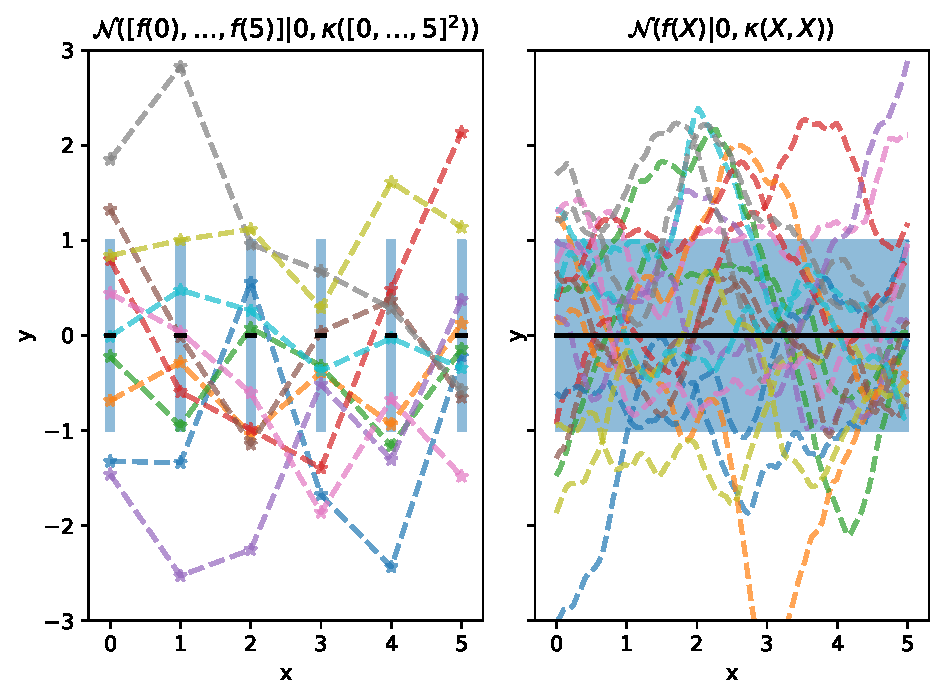
\includegraphics[width = \textwidth]{Pictures/GP_samples_mattern.pdf}
    \caption{Left: Samples from $\mathcal{N}(\textbf{f}|0,\kappa(x_1,\dots, x_{11}))$ where
    $x_i= 0.5(i-1)$. Illustration that a samples from a Gaussian process is just
    samples from the multivariate normal distribution. We could potentially choose
    $\textbf{x}$ to be all of the real line, which will give us the GP - an infinitely
    large multivariate normal distribution (right).}
    \label{GP_illustration}
\end{figure}

\subsection{Exact predictive distribution}
What we want is the predictive posterior distribution, of a new point $p(y_*|x_*, \mathcal{D})$, i.e. by marginalizing 
out the random variabel $f_* := f(x_*)$, 
\begin{equation}\label{GP_predictive}
    p(y_*|x_*,\mathcal{D}) = \int \mathcal{N}(y_*|f_*, \sigma^2) p(f_*|\mathcal{D})df_*
\end{equation}
where we assume that $\epsilon$ from \ref{..} is a Gaussian with zero mean and variance $\sigma^2$.
We will soon see that the posterior $p(f_*|\mathcal{D})$ is also a normal distribution 
with mean $\mu_*$ and variance $\sigma^2_*$ so
using <trick> we end up with the distribution. 
$$p(y_*|x_*,\mathcal{D}) = \mathcal{N}(y_*|\mu_*,\sigma^2_*+\sigma^2)$$
% where $\mu_* = E_{p(f_*|\mathcal{D})}[f_*]$ and $\sigma^2_* =
% V_{p(f_*|\mathcal{D})}[f_*]$

So now want to calculate $p(f_*|\mathcal{D})$, this can be done using the neat properties of Gaussian
distributions.  
\subsubsection{Posterior function distribution}
From observing the data $\mathcal{D} = \{x_1,y_1, \dots , x_n,y_n\} = (\textbf{x}, \textbf{y})$, we define the noisefree
predictions as $\textbf{f} = [f(x_1), \dots, f(x_n)]$ and marginalize them out in the following way, 
\begin{equation}\label{posterior_function_new}
    p(f_*|\mathcal{D})= \int p(f_*|\textbf{x}, \textbf{f})p(\textbf{f}|\mathcal{D})d\textbf{f}.
\end{equation} 
From \eqref{} we already have $p(f_*|\textbf{x}, \textbf{f}) = \mathcal{N}()$ so we just need to
calculate the posterior $p(\textbf{f}|\mathcal{D})$, this is done through the prior and likelihood, 
$$p(\textbf{f}|\mathcal{D}) \propto p(\textbf{f}|\textbf{x}) p(\textbf{y}|\textbf{f}).$$ 
As mentioned $f(\cdot)$ is the noisefree prediction, i.e. $y
= f(x)+ \epsilon$. So assuming iid data, and that $\epsilon$ is additive Gaussian
noise with variance $\sigma^2$, we get the likehood, 
\begin{align*}
    p(\textbf{y}|\textbf{x}, \textbf{f}) = \prod_{i=1}^n p(y_i|x_i,\textbf{f}_i) = \prod_{i=1}^n \mathcal{N}(y_i|\textbf{f}_i,\sigma^2) = \mathcal{N}(\textbf{y}|\textbf{f},\sigma^2 I)
\end{align*}
from \eqref{} the prior of $\textbf{f}$ is defined using similarities between it corresponding $\textbf{x}$, 
$p(\textbf{f}|\textbf{x}) = \mathcal{N}(\textbf{f}|\textbf{0},c(\textbf{x}, \textbf{x}))$
so we the posterior is given as, 
\begin{align*}
    p(\textbf{f}|\mathcal{D}) &\propto \mathcal{N}(\textbf{f}|\textbf{0}, c(\textbf{x}, \textbf{x})) \mathcal{N}(\textbf{y}|\textbf{f},\sigma^2 I)
\end{align*}
now, since this is a product between two Gaussians using \ref{} we have that the posterior is the following Gaussian: 
\begin{equation*}
    p(\textbf{f}|\mathcal{D}) = \mathcal{N}(\textbf{f}|M^{-1} \sigma^{-2}\textbf{y}, M^{-1}) \hspace{0.5cm}M := c(\textbf{x}, \textbf{x})^{-1}+\sigma^{-2} I_n
\end{equation*}

Finally, we see that both terms in the integral \eqref{posterior_function_new}, are related such
that it is possible to use \eqref{marginal_distribution} for arriving at (we define $A :=  c(x_*,
x_*)^{-1} c(x_*, \textbf{x})$), 
\begin{align*}
    p(f_*|\mathcal{D}) &= \mathcal{N}(f_*|\mu_*,\sigma_*^2 )\\
    \mu_* &=  AM^{-1}\sigma^{-2}\textbf{y}\\
    \sigma_*^2 &=  c(x_*, x_*)^{-1}+AM^{-1}A^T)
\end{align*}
We now have a fully specified Gaussian process posterior function, which we sample from 
in figure


\begin{figure}[h]
    \centering
    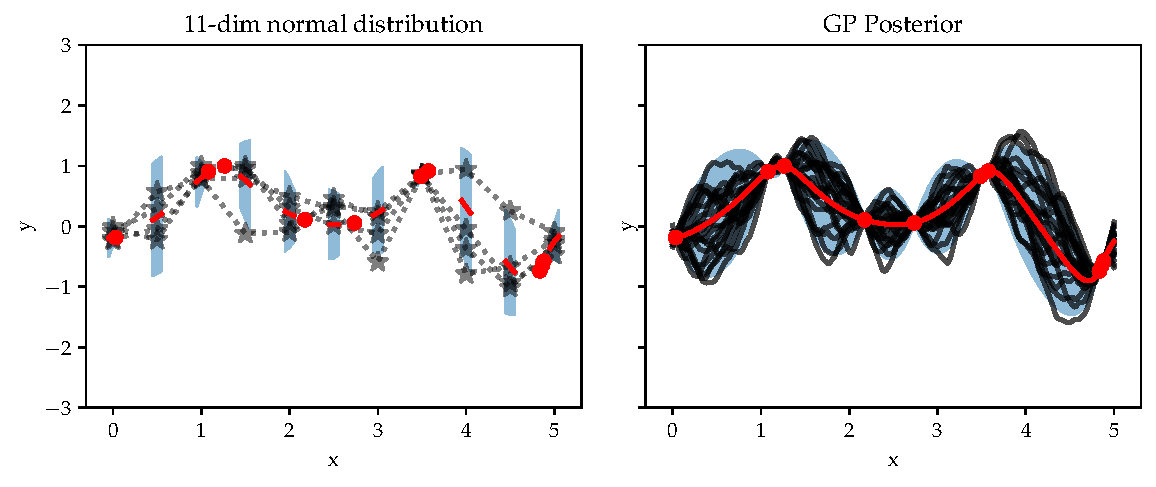
\includegraphics[width = \textwidth]{Pictures/GP2_samples_mattern.pdf}
    \caption{Left: Samples from posterior function distribution for
    $\mathcal{N}(\textbf{f}_*|m(\textbf{x}),V(\textbf{x}))$ where $\textbf{x} = \{x_1,\dots, x_{11}\}$
    and $x_i= 0.5(i-1)$. Illustration that a samples from a Gaussian process is just samples from
    the multivariate normal distribution. We could potentially choose $\textbf{x}$ to be all of the
    real line, which will give us the GP - an infinitely large multivariate normal distribution.}
    \label{GP_illustration2}
\end{figure}



\begin{testexample2}[Trick with normal distributions [from Bishops book?]]
    Given a marginal Gaussian distribution of $x$ and a conditional Gaussian distribution
    of $y$ given $x$ of the form, 
    \begin{align*}
        p(x) &= \mathcal{N}(x|\mu, \Lambda^{-1})\\
        p(y|x) &= \mathcal{N}(x|Ax+b, L^{-1})
    \end{align*}
    then the marginal distribution of $y$ and the conditional distribution of $x$ given $y$
    have the form, 
    \begin{align}
        p(y) &= \mathcal{N}(y|A\mu+b,L^{-1}+A \Lambda^{-1}A^T) \label{marginal_distribution}\\
        p(x|y) &= \mathcal{N}(x|\Gamma \mu+\Gamma [A^TL(y-b)],\Gamma )\\
        \Gamma &:= (\Lambda +A^TLA)^{-1}
    \end{align}
\end{testexample2}




\subsection{Learning - Emperical bayes inference}

The Gaussian process does contain some hyperparameters, a variance $\sigma^2$ and kernel parameters. 
Very often GP hyperparameters are chosen using Emperical bayes, which is simply to choose
the hypter parameters, which maximize the marginalized likehood,  
$$\nu = \argmin_{\nu} p(\textbf{y}|\textbf{x}, \nu)$$
where for a Gaussian process the marginal is given as 
\begin{align*}
    p(\textbf{y}|\textbf{x}, \nu) &= \int  p(\textbf{y}, \textbf{f}|\textbf{x}, \nu) d\textbf{f}\\
    &= p(\textbf{y}|\textbf{f},\nu)p(\textbf{f}|\textbf{x},\nu) d\textbf{f}
\end{align*}
where  $p(\textbf{y}|\textbf{f},\nu) = \mathcal{N}(\textbf{y}|\textbf{f},\sigma^2)$ and the prior is
just the Gaussian $p(\textbf{f}|\textbf{x},\nu) = \mathcal{N}(\textbf{f}|0, c_{\nu}(\textbf{x}, \textbf{x}))$
And now we can easily perform the integration using <...>, 
$$p(\textbf{y}|\textbf{x}, \nu) = -\frac{1}{2}[(y-\mu)^T (\Sigma+N)^{-1}(y-\mu)+ \log |\Sigma+N|+n \log 2\pi]$$

we can define the predictive prior distribution, in the same way as \eqref{GP_predictive}, we have that
$p(\textbf{f}| \textbf{x}) = \mathcal{N}(\textbf{f}|0, c(\textbf{x},\textbf{x}))$, thereby, 
\begin{equation}\label{GP_predictive_prior}
    p(\textbf{y}|\textbf{x}) = \int \mathcal{N}(\textbf{x}|\textbf{f}, I\sigma^2) p(\textbf{f}|\textbf{x})d\textbf{f}
\end{equation}
Using ... we arrive at 
just observe that $p(\textbf{y}|\textbf{x}) = \mathcal{N}(\textbf{y}|0, c(\textbf{x},\textbf{x})+ \sigma^2)$



\todo{Model assessment becomes trivial in light of the model posterior if we
simply establish preferences over models according to their posterior
probability. When using the uniform model prior (4.6)
 the model posterior is proportional to the marginal likelihood alone,
which can be then used directly for model assessment. ??! Youtube - good video! Go through that!}

\begin{figure}[H]
    \centering
    \begin{minipage}[b]{0.49\textwidth}
     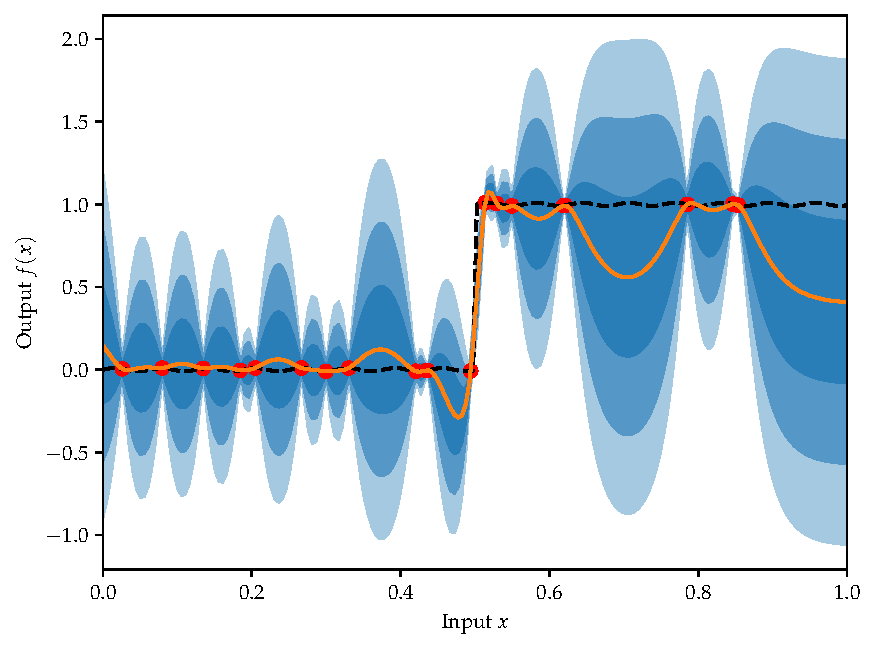
\includegraphics[width=\textwidth]{Pictures/GP_vs_BNN1.pdf}
    \end{minipage}
    \hfill
    \begin{minipage}[b]{0.49\textwidth}
      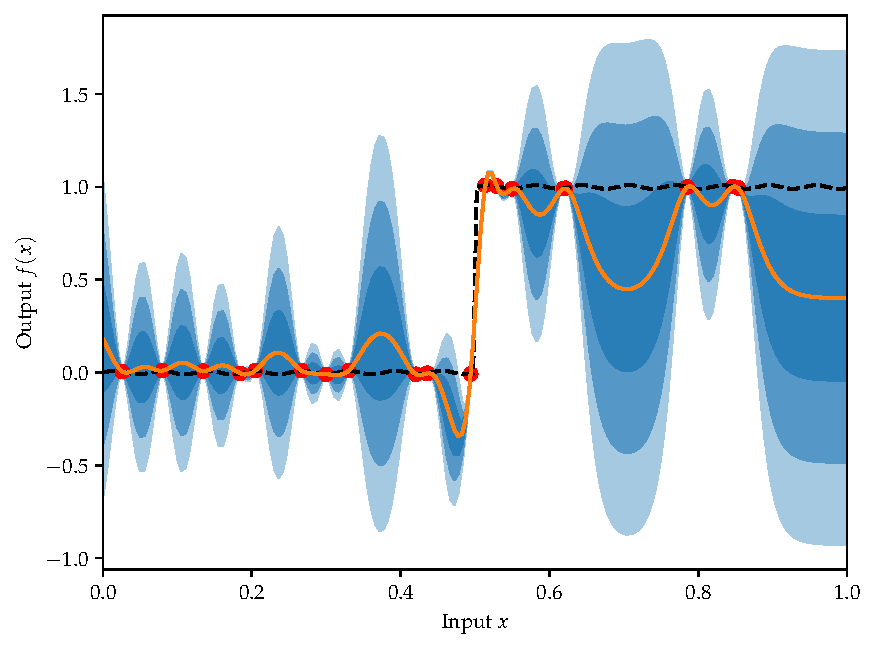
\includegraphics[width=\textwidth]{Pictures/GP_vs_BNN1_b.pdf}
     \end{minipage}
     \caption{There is large difference beween the two GPs the different lenght scales in the kernel
     matters a lot. Left is chosen 9 out of 10 times, when minimizing the }
\end{figure}
